
\chapter{从其他格式导入/导出}
\label{cha:pgfplots:importexport}

{
\tikzset{external/figure name/.add={}{importexport_}}

本章介绍如何把单个图导出为独立的 \pdf{} 图形文件（或 \eps{} 图形文件）。此外，还介绍了一个 Matlab$^\text{\textregistered}$ 脚本，可用于把 Matlab 图转换为 \PGFPlots{}。


\section[导出为 PDF/EPS]{导出为 {\normalfont\pdf{}/\eps{}}}
\label{sec:pgfplots:export}

可以使用 \pgfname{} 和/或 \Tikz{} 的例程，把图导出为独立的 \pdf{} 文档。


\subsection{使用 \Tikz 的自动外部化框架}

\begin{pgfplotslibrary}{external}
\pgfkeys{/pdflinks/search key prefixes in/.add={/tikz/external/,}{}}
    |external| 库提供了一种便捷的方法，把每个独立的 |tikzpicture| 导出为单独的~|.pdf|（或~|.eps|）。后续的 \LaTeX{} 运行将直接包含这些图形，从而显著减少排版时间。

    该库也可以用于把文档提交给那些甚至没有安装 \PGFPlots{} 或 \Tikz{} 的作者。


    \paragraph{技术前言：}

    |external| 库由 Christian Feuersänger（\PGFPlots 的作者）编写。它已作为通用库贡献给 \Tikz{}，因此完整的参考文档以及所有调节选项可参见~\cite[Section ``Externalization Library'']{tikz}。命令 |\usepgfplotslibrary{external}| 实际上只是一个包装，它加载 |\usetikzlibrary{external}|；如果因为所安装的 \pgfname{} 版本至多为 $2.00$ 而该库尚不存在，则加载 \PGFPlots{} 自带的一个副本。

    |external| 库的设计使得对文档本身\emph{无需做任何改动}。其思路如下：
    %
    \begin{enumerate}
        \item 每一个 |\begin{tikzpicture}| $\dotsc$ |\end{tikzpicture}| 都会得到一个文件名。文件名既可以用 |\tikzsetnextfilename|\marg{output file name} 手动指定，也可以自动生成；自动生成时使用 \meta{tex file name}|-figure|\meta{number}，其中 \meta{number} 递增。

        \item 该库通过 \TeX{} 的 write18 系统调用，自动以形如 |pdflatex --jobname |\meta{output file name} 的命令写出生成的图片。这与调用 |gnuplot| 所用的是同一套框架。
    \end{enumerate}
    %
    唯一必要的步骤是使用

    \pgfmanualpdflabel{\textbackslash tikzexternalize}{}%
    |\usepgfplotslibrary{external}|

    |\tikzexternalize|

    \noindent 在文档导言区的某处（与系统相关的配置选项见下文）。文档无需再做其他修改。假设我们有一个名为 |test.tex| 的文件：
    %
\begin{codeexample}[code only]
\documentclass{article}
\usepackage{pgfplots}
    \usepgfplotslibrary{external}
    \tikzexternalize% activate externalization!
\begin{document}
    \begin{figure}
        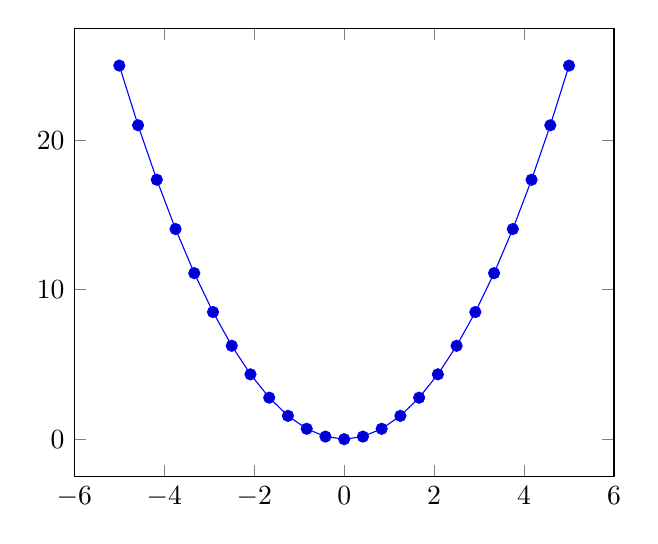
\begin{tikzpicture}
            \begin{axis}
                \addplot {x^2};
            \end{axis}
        \end{tikzpicture}
        \caption{Our first external graphics example}
    \end{figure}

    \begin{figure}
        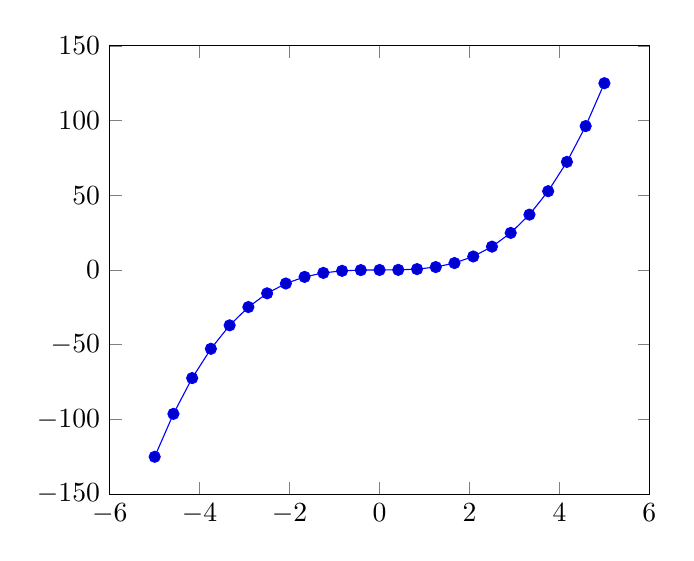
\begin{tikzpicture}
            \begin{axis}
                \addplot {x^3};
            \end{axis}
        \end{tikzpicture}
        \caption{A second graphics}
    \end{figure}
\end{document}
\end{codeexample}
    %
    \noindent 要启用系统调用，我们输入
    %
\begin{codeexample}[code only]
pdflatex -shell-escape test
\end{codeexample}
    %
    \noindent 之后 \LaTeX{} 会自动生成所需的图形文件 |test-figure0.pdf| 和 |test-figure1.pdf|。之后每次调用 |pdflatex| 都会直接使用 |\includegraphics|，不再重新处理 |tikzpicture| 本身（对于 MiK\TeX{}，需要不同的命令行开关，参见 |shell escape| 选项）。

    如果某个图需要重新生成，只需删除全部或部分图形文件并重新生成即可。另一种方式是在文档的某处使用 |\tikzset{external/force remake}|，之后每一个图都会自动重新生成。

    外部化图的文件名有三种修改方式：
    %
    \begin{itemize}
        \item 使用 |prefix| 修改整体文件名前缀，
        \item 使用 |\tikzsetnextfilename| 修改单个图的文件名，
        \item 使用 |figure name| 修改一组图的文件名。
    \end{itemize}

    \begin{key}{/tikz/external/prefix=\marg{file name prefix} (initially empty)}
        |\tikzsetexternalprefix|\marg{file name prefix} 的快捷方式，见下文。
    \end{key}

    \begin{command}{\tikzsetexternalprefix\marg{file name prefix}}
        为所有文件名指定一个公共前缀。例如，
        %
\begin{codeexample}[code only]
\tikzsetexternalprefix{figures/}
\end{codeexample}
        %
        会把 |figures/| 加到每一个外部图形文件名之前。
    \end{command}

    \begin{command}{\tikzsetnextfilename\marg{file name}}
        为\emph{下一个} \tikzname{} 图或 |\tikz| 短命令设置文件名。它\emph{只}对下一个图生效。

        没有显式指定文件名的图会自动生成文件名。

        请注意，|prefix| 仍然会被加到 \meta{file name} 之前。
        %
\begin{codeexample}[code only]
\documentclass{article}
% main document, called main.tex
\usepackage{tikz}
    \usepgfplotslibrary{external}
    \tikzexternalize[prefix=figures/]% activate with a name prefix
\begin{document}
\tikzsetnextfilename{firstplot}
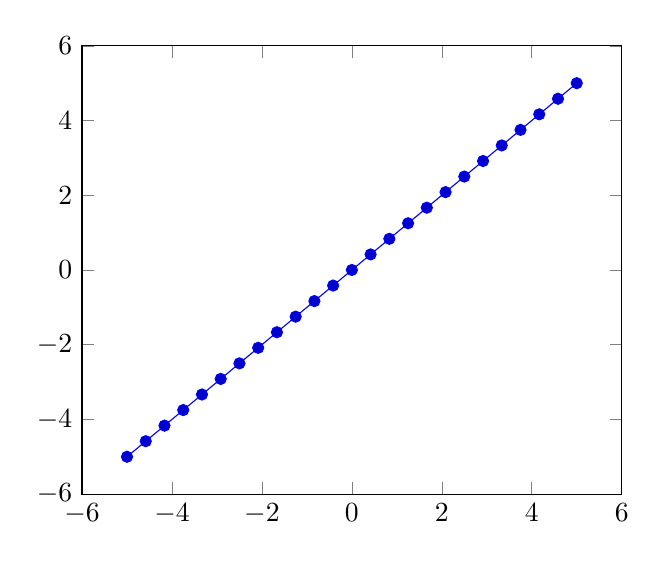
\begin{tikzpicture} % will be written to 'figures/firstplot.pdf'
    \begin{axis}
        \addplot {x};
    \end{axis}
\end{tikzpicture}


\begin{tikzpicture} % will be written to 'figures/main-figure0.pdf'
   \draw [help lines] (0,0) grid (5,5);
\end{tikzpicture}
\end{document}
\end{codeexample}

\begin{codeexample}[code only]
pdflatex -shell-escape main
\end{codeexample}
        %
    \end{command}

    \begin{key}{/tikz/external/figure name=\marg{name}}
        与 |\tikzsetfigurename|\marg{name} 相同。
    \end{key}

    \begin{command}{\tikzsetfigurename\marg{name}}
        修改\emph{之后所有}图的名称。在文档编写过程中，可以通过
        |\tikzset{external/figure name|=\marg{name}|}| 来修改 |figure name|。每一个不同的 \meta{name} 都会使用一个独立的计数器，每个计数器都从
        $0$ 开始。\footnote{这些计数器存储在不同的\emph{宏}中。换句话说：不需要使用 \TeX{} 寄存器。}

        |prefix| 的值会在 |figure name| 求值之后再应用。
        %
\begin{codeexample}[code only]
\documentclass{article}
% main document, called main.tex
\usepackage{tikz}
    \usepgfplotslibrary{external}
    \tikzexternalize% activate externalization!
\begin{document}
% will be written to 'main-figure0.pdf'
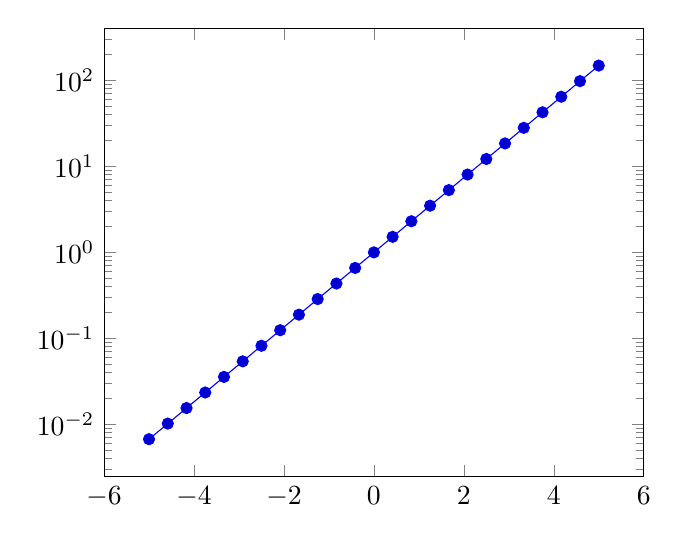
\begin{tikzpicture}
    \begin{semilogyaxis}
        \addplot {exp(x)};
    \end{semilogyaxis}
\end{tikzpicture}

{
    \tikzset{external/figure name={subset_}}
    A simple image is \tikz \fill (0,0) circle(5pt);. % will be written to 'subset_0.pdf'

    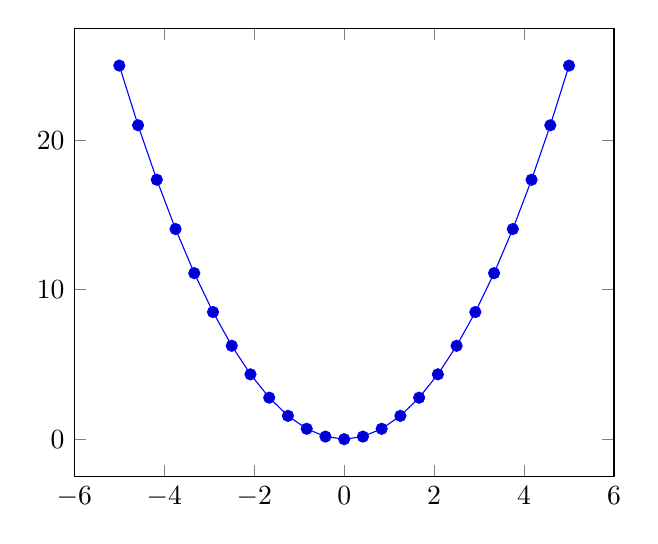
\begin{tikzpicture} % will be written to 'subset_1.pdf'
        \begin{axis}
            \addplot {x^2};
        \end{axis}
    \end{tikzpicture}
}% here, the old file name will be restored:

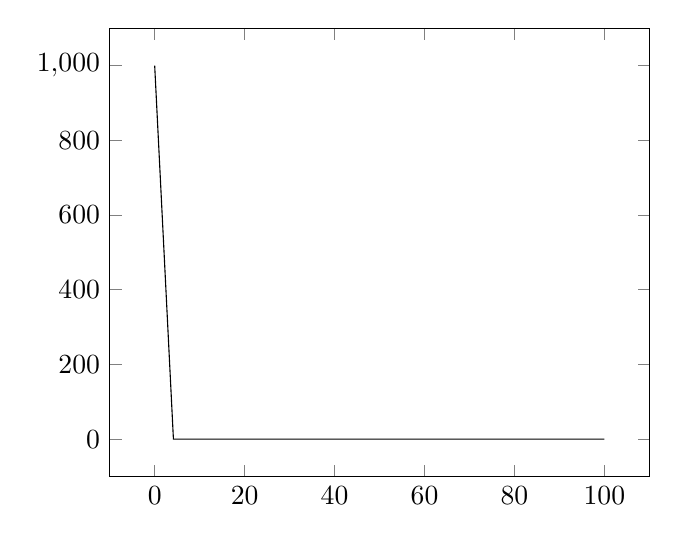
\begin{tikzpicture} % will be written to 'main-figure1.pdf'
    \begin{axis}
        \addplot[domain=1e-3:100] {1/x};
    \end{axis}
\end{tikzpicture}
\end{document}
\end{codeexample}
        %
        |figure name| 的作用域在下一个右花括号处结束（与 |\tikzset| 设置的所有值一样）。

            \medbreak
        备注：使用
        |\tikzset{external/figure name/.add=|\marg{prefix}\marg{suffix}|}| 可以在 |figure name| 的实际值前添加一个 \meta{prefix}、在末尾追加一个 \meta{suffix}。这对于类似下面这样的场景可能有用：
        %
\begin{codeexample}[code only]
\tikzset{external/figure name=main}

% uses main_0.pdf, main_1.pdf, ...

\chapter{The first section}
{\tikzset{external/figure name/.add={}{_firstsection}}
    ...
    % uses main_firstsection_0.pdf, main_firstsection_1.pdf, ...
}

\chapter{The second section}
{\tikzset{external/figure name/.add={}{secondsection_}}
    ...
    % uses main_secondsection_0.pdf, main_secondsection_1.pdf, ...
    \section{Second subsection}
    {\tikzset{external/figure name/.add={}{sub_}}
        ...
        % uses main_secondsection_sub_0.pdf, main_secondsection_sub_1.pdf, ...
    }
    % uses main_secondsection_2.pdf, main_secondsection_3.pdf, ...
}
\end{codeexample}
    \end{command}

    \begin{command}{\tikzappendtofigurename\marg{suffix}}
        在 |figure name| 的实际值之后追加 \meta{suffix}。

        它是
        |\tikzset{external/figure name/.add={}|\marg{suffix}|}| 的快捷方式（即使没有安装 \tikzname{} 也支持此快捷方式，见下文）。
    \end{command}


    \paragraph{\textsc{eps} 输出或 MiK\TeX{} 的配置选项：}

    由于 |external| 库通过系统调用来工作，因此需要根据本地系统进行调整。对于 MiK\TeX{} 这是必要的，因为它使用不同的选项来启用这些系统调用。对于 \textsc{eps} 输出也是必要的，因为这涉及到一组不同的工具。

    请注意，\emph{最重要的部分}是启用系统调用。通常的做法是用 |pdflatex -shell-escape| 或 |pdflatex -enable-write18|（MiK\TeX{}）来排版你的文档。这些选项\emph{需要在你的 \TeX{} 编辑器中配置}。除这一步之外，你可能还希望配置系统调用：

    \begin{key}{/tikz/external/system call=\marg{template}}
    \label{extlib:systemcall:option}
        用于生成系统调用的模板字符串。在 \meta{template} 内部，宏 |\image| 可以作为占位符，表示即将生成的图片；而 |\texsource| 包含主文件名（实际上它包含 |\input|\marg{main file name}，但这无关紧要）。

        默认值为
        %
\begin{codeexample}[code only]
\tikzset{external/system call={pdflatex \tikzexternalcheckshellescape -halt-on-error
    -interaction=batchmode -jobname "\image" "\texsource"}
\end{codeexample}
        %
        \noindent 其中 \declareandlabel{\tikzexternalcheckshellescape} 仅在当前文档是用 |-shell-escape| 排版时，才会插入配置键 |shell escape| 的值。\footnote{请注意，对于默认配置而言这总是成立的。这一安全考虑主要针对 \texttt{mode=list and make}，它\emph{不}需要 shell escape 也能工作。}

        对于 |eps| 输出，你可以（并且需要）使用
        %
\begin{codeexample}[code only]
\tikzset{external/system call={latex \tikzexternalcheckshellescape -halt-on-error
    -interaction=batchmode -jobname "\image" "\texsource" &&
    dvips -o "\image".ps "\image".dvi}}
\end{codeexample}

        参数 \meta{template} 会用 |\edef| 展开，因此所有控制序列都会被展开。在这一求值过程中，`|\\|' 会变成一个普通反斜杠 `|\|'。此外，如果某些宏包把双引号 `|"|'、单引号 `|'|'、分号和短横线 `|-|' 用作宏，它们也会被转换为普通字符。例如，这保证了与 |german| 宏包的兼容性。
    \end{key}

    \begin{key}{/tikz/external/shell escape=\marg{command-line arg} (initially -shell-escape)}
        包含启用 |\write18| 特性的 |latex| 命令行选项。

        对于 \TeX{}Live，是 |-shell-escape|。对于 MiK\TeX{}，系统使用 |-enable-write18|。
    \end{key}


    \paragraph{对外部文件中标签与引用的支持}

    |external| 库对外部文件中的 |\label| 和 |\ref|（以及其他通常会在 |.aux| 文件中保存信息的命令）提供了额外的支持。

    然而，当你尝试使用下面两种情况时，仍有几点需要注意：
    %
    \begin{enumerate}
        \item[a)] 在外部化图形中引用主文档中的某个对象；或
        \item[b)] 在外部化图形中使用 |\label|，而该标签在主文档中被引用。
    \end{enumerate}

    对于情况 a)，外部化图形中的 |\ref| \emph{仅}在你\emph{手动}发出所需的系统调用、或通过 |make| 时才能工作。初始配置 |mode=convert with system call| \emph{不}支持 |\ref|。但你可以复制并粘贴由 |mode=convert with system call| 生成的系统调用，然后手动执行。原因在于 |\ref| 信息存储在主 |.aux| 文件中——但在调用 |mode=convert with system call| 时，该辅助文件还没有完全写完（存在竞争条件）。请注意，|\pageref| 不被支持（抱歉）。因此：如果外部图形中含有 |\ref|，请考虑使用 |mode=list and make|，或复制并粘贴该图的系统调用并手动执行。

    情况 b) 由外部库自动实现。具体来说，外部化图形中的 |\label| 会使外部库为每一张外部图生成单独的辅助文件。这些文件名为 \meta{imagename}|.dpth|。扩展名 |.dpth| 表示该文件还包含图片的深度（即 \tikzname 的 |baseline| 键）。此外，本应写入 |.aux| 文件的任何内容都会被重定向到 |.dpth| 文件——但仅限发生在外部化 |tikzpicture| 环境内部的内容。当主文档加载该图时，会把 |.dpth| 文件的内容拷贝到主 |.aux| 文件中。之后对主文档的后续编译就会包含外部的 |\label| 信息。换句话说，外部图形中的 |\label| 需要遵循下面的工作流程：
    %
    \begin{enumerate}
        \item 外部图形需要连同其 |.dpth| 一起生成（通常由 \tikzname 自动完成）。
        \item 主文档包含该外部图形，并把 |.dpth| 的内容拷贝到自己的主 |.aux| 文件中。
        \item 主文档需要再编译一次，以重新读取其 |.aux| 文件。\footnote{请注意，在 \LaTeX{} 中，无法在 \texttt{\textbackslash begin\{document\}} 之后激活辅助文件的内容。}
    \end{enumerate}
    %
    还有一种特殊情况：当 |\label|/|\ref| 是由 |tikzpicture| 绘制出来的时候。例如图例中的 |\ref| 图片，或 |\pgfplotslegendfromname| 特性。在这种情况下，你需要按照情况 a) 的方式处理，因为 |mode=convert with system call| 本身无法处理这些内容。

    换句话说：外部文档中的 |\label| 可以自动工作，只要把主文档多编译几次即可。|\ref| 则可能需要像上面情况 a) 那样手动调整。


    \paragraph{操作模式}

    \begin{key}{/tikz/external/mode=\mchoice{convert with system call,list and make,$\dotsc$} (initially convert with system call)}
        该键用于修改默认的操作模式。有若干种选项，全部详见
        ~\cite[Section ``Externalization Library'']{tikz}。其中最常用的大概是初始配置 |convert with system call| 以及专门选项 |list and make|。

        选项 |list and make| 配置该库去检查外部图形是否已经存在，并使用已存在的图形。如果图形不存在，该库会\emph{跳过}该图。但它同时还会生成一个 |makefile| 用于生成这些图形，以及一份所有必需图形文件的清单。

        不强制要求使用 |make|：该库只期待你以某种方式生成图片，并不关心「如何生成」。使用
        |make -f |\meta{name-of-tex-file}|.makefile -j 2| 可以并行执行，这确实可能是一个不错的选择。此外，makefile 还支持文件依赖：如果你的某个数据表已更新，外部图形会自动重新生成。\PGFPlots{} 会把任何文件依赖（输入文件和数据表）告知外部库。

        这两种模式具有如下特点：
        %
        \begin{enumerate}
            \item |convert with system call| 是全自动的，会即时完成所有工作。但它\emph{无法}处理外部图片中的 |\ref| 和/或 |\label| 信息。
            \item |list and make| 需要手动（手动发出系统调用）或半自动转换（使用生成的 \meta{main}|.makefile|），并多次运行 |pdflatex|。生成的 Makefile 可以并行处理。此外，|list and make| 对 |\ref| 和 |\label| 提供\emph{完整支持}：在外部化图形中定义的任何 |\label| 仍然可供主文档使用。

                如果你有使用 |legend to name| 的图例，或使用 |\label|/|\ref|，那么你需要先生成定义该 |\label|（或 |legend to name|）的图形，然后在主文档上运行 |pdflatex| 两次。之后就可以把该图例图形外部化了。
        \end{enumerate}
    \end{key}

    完整的参考文档以及其余选项记录在~\cite[``Externalization Library'']{tikz} 中。该参考还包含关于以下内容的信息：
    %
    \begin{itemize}
        \item 如何使用
            |\tikzset{external/|\declareandlabel{force remake}|}| 和
            |\tikzset{external/|\declareandlabel{remake next}|}| 来重新生成选定的图，
        \item 如何用
            |\tikzset{external/|\declareandlabel{export}|=false}| 部分禁用外部化，或用
            |\tikzexternaldisable| 完全禁用，
        \item 如何使用
            |\tikzset{external/optimize command away=\myExpensiveMacro}| 优化转换过程的速度，
        \item 如何用
            |\tikzpicturedependsonfile|\marg{name} 和/或
            |\tikzexternalfiledependsonfile|\marg{external file}\marg{name} 添加更多重新生成的依赖，
        \item 如何启用 |png| 导出的示例，
        \item 如何在未安装 \pgfname{} 的情况下排版此类文档，或
        \item 如何应对 |.pdf| 图片与边界框限制的变通方法。 \index{External Graphics!Bounding Box Issues}
            \index{Bounding Box Control!Image Externalization Problems}
    \end{itemize}


    \paragraph{在未安装 {\normalfont\pgfname} 或 {\normalfont\PGFPlots} 的情况下使用该库}

    有一个小型替换宏包 \declareandlabel{tikzexternal.sty}，可以在每个图都导出之后使用。思路是注释掉 |\usepackage{tikz}| 和 |\usepackage{pgfplots}|，改为写 |\usepackage{tikzexternal}|：
    %
\begin{codeexample}[code only]
% \usepackage{tikz}
% \usepackage{pgfplots}
\usepackage{tikzexternal}
    \tikzexternalize% activate externalization
\begin{document}
    \begin{tikzpicture}
        ...
    \end{tikzpicture}
...
\end{document}
\end{codeexample}
    %
    你不需要安装 \pgfname{}、\tikzname{} 或 \PGFPlots{}。你需要的是 |tikzexternal.sty| 以及所有生成的图（包括图片文件 `|.pdf|'，以及包含 |baseline| 选项信息的 `|.dpth|' 文件）。|tikzexternal.sty| 随 \pgfname{} 一起发布，位于目录
    %
\begin{codeexample}[code only]
latex/pgf/utilities/tikzexternal.sty
\end{codeexample}
    %
    同时 \PGFPlots{} 也附带了一份副本：
    %
\begin{codeexample}[code only]
tex/generic/pgfplots/oldpgfcompatib/pgfplotsoldpgfsupp_tikzexternal.sty
\end{codeexample}
    %
    只需把该文件拷贝到你的目录下，并将其重命名为 |tikzexternal.sty|。


    \paragraph{注意：}

    这个小型替换宏包不支持键值接口。因此，必须用 |\tikzsetexternalprefix| 代替 |prefix| 选项，用 |\tikzsetfigurename| 代替 |figure name| 选项，因为在这种上下文中 |\tikzset| 不可用。另外，如果你之前用过 |\pgfplotsset|，可能还需要定义一个空的宏 |\pgfplotsset|。
\end{pgfplotslibrary}


\subsection[手动使用 PGF 外部化框架]{手动使用 {\normalfont\pgfname} 的外部化框架}

把 \TeX{} 图导出为独立图形文件的另一种方法是使用 \pgfname{} 的外部化框架。它需要更多工作，但比 |external| 库更通用。基本思路是用如下命令把希望导出的部分封装起来：

\declareandlabel{\beginpgfgraphicnamed}\marg{output file name}

\meta{picture contents}

\declareandlabel{\endpgfgraphicnamed}.

\noindent 此外，还需要在导言区用如下命令告知 \pgfname{} 主文档的名称：

\declareandlabel{\pgfrealjobname}\marg{the real job's name}

\noindent 在导言区。这会启用两种不同的模式：
%
\begin{enumerate}
    \item 第一种是正常排版模式。\LaTeX{} 会检查是否存在名为 \meta{output file name}、且带有某种可接受扩展名的文件——如果存在，则用 |\pgfimage| 包含该图形文件，并跳过 \meta{picture contents}。如果该文件不存在，则正常排版 \meta{picture contents}。当 |\jobname| 等于 \meta{the real job's name} 时，使用此模式。
    \item 第二种模式在 |\jobname| 等于 \meta{output file name} 时启用，它进入「转换模式」，用于写出图形文件 \meta{output file name}。此时，\emph{只}把 \meta{picture contents} 写入 |\jobname|，\LaTeX{} 的其余部分照常处理，但会被静默丢弃。

        对于每一个外部化图形文件，都需要手动用
        |pdflatex --jobname |\meta{output file name} 来启动此模式。
\end{enumerate}
%
下面是一个完整的示例。
%
\begin{codeexample}[code only]
\documentclass{article}
\usepackage{pgfplots}
    \pgfrealjobname{test}
\begin{document}
    \begin{figure}
        \beginpgfgraphicnamed{testfigure}
            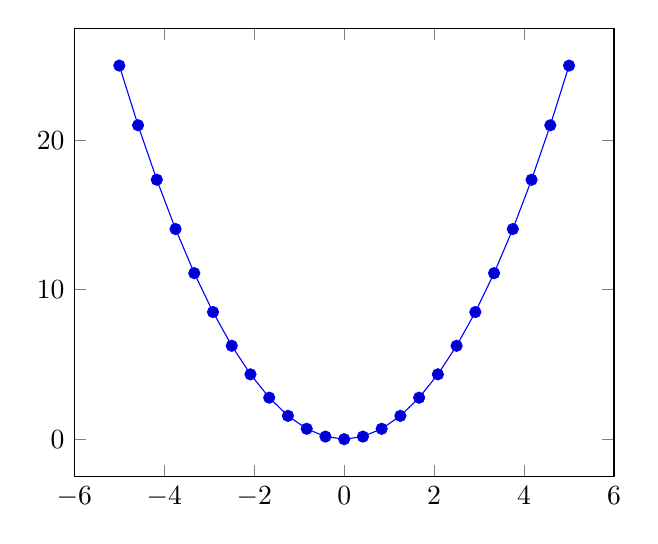
\begin{tikzpicture}
                \begin{axis}
                    \addplot {x^2};
                \end{axis}
            \end{tikzpicture}
        \endpgfgraphicnamed
        \caption{Our first external graphics example}
    \end{figure}

    \begin{figure}
        \beginpgfgraphicnamed{testfigure2}
            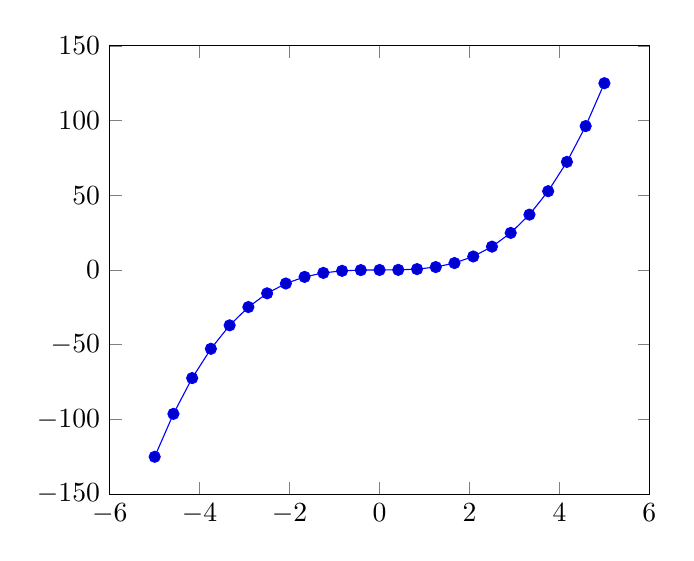
\begin{tikzpicture}
                \begin{axis}
                    \addplot {x^3};
                \end{axis}
            \end{tikzpicture}
        \endpgfgraphicnamed
        \caption{A second graphics}
    \end{figure}
\end{document}
\end{codeexample}
%
\noindent 该文件名为 |test.tex|，我们用如下命令处理它（例如）：
%
\begin{codeexample}[code only]
pdflatex test
\end{codeexample}
%
\noindent 现在我们输入
%
\begin{codeexample}[code only]
pdflatex --jobname testfigure test
pdflatex --jobname testfigure2 test
\end{codeexample}
%
\noindent 进入转换模式。最后这两次调用\emph{只}会把我们命名的图形环境内容写入各自的输出文件 |testfigure.pdf| 和 |testfigure2.pdf|：一个对应 \meta{testfigure}，另一个对应 \meta{testfigure2}。

总之，需要 |\pgfrealjobname|，并对每一个外部化图形环境调用
|pdflatex --jobname |\meta{graphics file}。请注意，必须使用上面给出的语法，\emph{不要}使用 |\begin{pgfgraphicnamed}|。

这些步骤在~\cite{tikz} 的 Section``Externalizing Graphics'' 中有更详细的说明。


\paragraph{注意：}

不要忘记正确的 |\pgfrealjobname| 语句！如果缺失，外部化将根本无法工作。如果写错，每次调用 \LaTeX{} 都会生成空的输出文件。

需要注意的是，这种图片外部化方法并不局限于 \Tikz{} 图环境。事实上，它会把起始与结束语句之间的所有内容都收集到外部文件中。这里隐含的假设是被封装的内容是一个盒子，但你也可以用类似 \LaTeX{} minipage 的方式（或使用 |\vbox|，它功能没那么强大，但对文档其余部分影响也更小）封装完整的段落。

\begin{key}{/pgf/images/aux in dpth=\mchoice{true,false} (initially false)}
    如果该布尔键被设为 |true|，则在外部图片内部生成的任何 |\label| 信息都会存储到前面提到的 |.dpth| 文件中。这样主文档就可以引用文档中被外部化部分的标签信息（尽管你可能需要多次运行 |latex|）。

    对 |\ref| 提供了标签支持，可能也包括 |\cite|。|\pageref| 命令只被部分支持。
\end{key}


\paragraph{在未安装 {\normalfont\pgfname} 的情况下使用该库}

只需把宏包 |\usepackage{tikz}| 和 |\usepackage{pgfplots}| 取消注释，改为使用
%
\begin{codeexample}[code only]
\long\def\beginpgfgraphicnamed#1#2\endpgfgraphicnamed{%
    \begingroup
    \setbox1=\hbox{\includegraphics{#1}}%
    \openin1=#1.dpth
    \ifeof1 \box1
    \else
        \read1 to\pgfincludeexternalgraphicsdp \closein1
        \dimen0=\pgfincludeexternalgraphicsdp\relax
        \hbox{\lower\dimen0 \box1 }%
    \fi
    \endgroup
}
\end{codeexample}
%
代替。这将包含生成的图形文件（并且会遵循 |.dpth| 文件中存储的 |baseline| 信息）。这样一来，你就不需要安装 \pgfname{} 或 \PGFPlots{}。详见~\cite{tikz} 的 Section``Externalizing Graphics''。


\section{从 Matlab 导入}

\subsection{从 Matlab 导入网格数据到 PGFPlots}
\label{sec:pgfplots:import:matlab}

虽然把 Matlab 向量写入文件很容易（使用 |save P.dat data -ASCII|），但导出网格数据就要复杂得多。

主要问题在于如何把网格结构告诉 \PGFPlots{}。

下面是实现这一任务的一个例子：在 Matlab 中，我们有网格数据 |X|、|Y| 和 |Z|，它们是大小相同的矩阵。例如，假设我们有
%
\begin{codeexample}[code only]
[X,Y] = meshgrid( linspace(-1,1,5), linspace(4,5,10) );
Z = X + Y;
surf(X,Y,Z)
\end{codeexample}
%
\noindent 作为数据。然后，我们可以生成一个 $N \times 3$ 的表，按列优先顺序包含所有单独的元素：
%
\begin{codeexample}[code only]
data = [ X(:) Y(:) Z(:) ]
% or -ascii
save P.dat data -ASCII
size(X)
ans =
   10.00    5.00
\end{codeexample}
%
\noindent 其中第二条命令把 $N \times 3$ 的表存入 |P.dat|。最后，我们可以在 \PGFPlots{} 中使用

|\addplot3[surf,mesh/rows=10,mesh/ordering=colwise,shader=interp] file {P.dat};|

来读取这些数据。我们需要提供行数（这里是 $10$）或列数——以及排序方式（对于 Matlab 矩阵是 |colwise|）。

在 \PGFPlots{} 中更快的另一种做法是：在 Matlab 中转置矩阵，并告诉 \PGFPlots{} 它们是按 |rowwise| 顺序排列的。这样，最后一步就变为
%
\begin{codeexample}[code only]
XX=X'; YY=Y'; ZZ=Z';
data = [ XX(:) YY(:) ZZ(:) ]
save P.dat data -ASCII
\end{codeexample}
%
\noindent 对应的 \PGFPlots{} 命令为

|\addplot3[surf,mesh/cols=10,mesh/ordering=rowwise,shader=interp] file {P.dat};|.


\subsection{matlab2pgfplots.m}

这是一个 Matlab$^\text{\textregistered}$ 脚本，尝试把 Matlab 图转换为 \PGFPlots{}。它要求 Matlab 版本 7.4（或更高）。


\paragraph{注意：}

该脚本已经严重过时，只支持 \PGFPlots{} 非常小的一个子集。你可以看看 |matlab2tikz|，这是 Nico Schlömer 编写的转换脚本，地址为

\url{http://www.mathworks.com/matlabcentral/fileexchange/22022-matlab2tikz}

\noindent 它同样使用 \PGFPlots{} 进行 \LaTeX{} 转换。

\medskip
|matlab2pgfplots.m| 的思路是
%
\begin{itemize}
    \item 以完整的 Matlab 图作为输入，
    \item 获取坐标轴标签、坐标轴缩放（对数或普通）以及图例条目，
    \item 获取所有绘图坐标
\end{itemize}
%
并写出一个等价的 \texttt{.pgf} 文件，用 \PGFPlots{} 来排版该图。

其目的\emph{不是}模拟 Matlab。它只是转换工作的第一步。在 Matlab 命令行输入
%
\begin{lstlisting}
> help matlab2pgfplots
\end{lstlisting}
%
在 Matlab 提示符下，可获得关于其特性与局限的更多信息。

该脚本仍处于实验阶段。


\subsection{matlab2pgfplots.sh}

一个 \texttt{bash} 脚本，简单地启动 Matlab 并运行
%
\begin{lstlisting}
    f=hgload( 'somefigure.fig' );
    matlab2pgfplots( 'outputfile.pgf', 'fig', f );
\end{lstlisting}
%
参见上面的 matlab2pgfplots.m。


\subsection{从 Matlab 导入颜色映射表}

有时你可能希望在 \PGFPlots{} 中复用 Matlab 的 |colormap|。下面是一个把 Matlab 颜色映射表转换为 \PGFPlots{} 的小脚本：
%
\begin{codeexample}[code only]
C = colormap;  % gets data of the current colormap.
% C = colormap(jet) % gets data of "jet"
eachnth = 1;
I = 1:eachnth:size(C,1); % this is nonsense for eachnth=1 -- but perhaps you don't want each color.
CC = C(I,:);
TeXstring = [ ...
 sprintf('\\pgfplotsset{\n\tcolormap={matlab}{\n') ...
 sprintf('\t\trgb=(%f,%f,%f)\n',CC') ...
 sprintf('\t}\n}\n') ]
\end{codeexample}


\section{SVG 输出}

可以把每一个 \Tikz{} 图都写入一个可缩放矢量图形（\texttt{.svg}）文件。这与 \PGFPlots{} 无关，它是 \PGF{} 的一个独立驱动。请参见~\cite[Section ``Producing HTML / SVG
Output'']{tikz}。


\section{在 Python 中生成 \PGFPlots{} 图形}

Mario Orne DÍAZ ANADÓN 贡献了一个小型 python 脚本 |pgfplots.py|，它提供了一个简单的接口，可以在 python 中生成 \PGFPlots{} 图。该脚本位于 \PGFPlots{} 安装目录下的
|pgfplots/scripts/pgfplots/pgfplots.py|；其文档可在该文件中找到。

}
